\section{Poisson's Equation and Laplace's Equation}
\subsection{The boundary value problem}
Many equations in mathematical physics can be
reduced to one of the form
\begin{definition}[Poisson's equation, Laplace's equation]
    The \textbf{Poisson's equation} is
    \[
      \nabla^2 \varphi = F,
    \]
    where $F$ is given and $\varphi$ is to be solved. When $ F=0 $, the equation becomes 
    \[
        \laplacian \varphi = 0,
    \]
    which is called the \textbf{Laplace's equation}.
\end{definition}

This equation either needs to be solved on all of $ \mathbb{R}^{n} $, or some domain $ \Omega \subseteq \mathbb{R}^{n} $, where $n=2,3$.

Physical problems involve boundary conditions, so to solve Poisson's equation we need to prescribe some boundary conditions for the function $\varphi$ on the boundary $\partial \Omega,$ or as $|\mathbf{x}| \rightarrow \infty$ if solving on all of $\mathbb{R}^{n}$. 

The \textbf{Dirichlet problem} for Poisson's equation is
\[
    \begin{cases}
        \nabla^{2} \varphi =F&\text {in } \Omega \\
        \varphi =f&\text {on } \partial \Omega\\
    \end{cases} 
\]
and the \textbf{Neumann problem} is
\[
    \begin{cases}
        \nabla^{2} \varphi =F  &\text {in } \Omega \\
        \dfrac{\partial \varphi}{\partial \mathbf{n}}=g & \text {on } \partial \Omega\\
    \end{cases} 
\]
Here we have used the normal derivative
\[
    \frac{\partial \varphi}{\partial \mathbf{n}} \equiv \mathbf{n} \cdot \nabla \varphi.
\]

It is important to interpret the boundary conditions in an appropriate way: we assume that $ \varphi $ \textit{continuously} approaches the boundary data as $\mathbf{x}\to\partial \Omega$, i.e. we assume that \textit{$\varphi$ and $\nabla \varphi$ are continuous on the set $\Omega \cup \partial \Omega$}.

\begin{remark}
    If $ \laplacian \varphi=0 $ in $ \Omega $, then $ \varphi $ needs to be well-defined on all of $ \Omega $. Don't fall into trap of assuming things like
    \[
        \laplacian\left( \frac{1}{|\mathbf{x}|} \right)=0,\quad \forall \mathbf{x}\in \mathbb{R}^{3}.
    \]
    It is only true for $\mathbf{x}\neq \mathbf{0}$ (check this). So when we’re talking about solutions to Laplace’s equation, we’re necessarily talking about functions which are non-singular. 
\end{remark}

\begin{example}
    Let $ r=|\mathbf{x}| $. Consider boundary value problem 
    \[\tag{$*$}
        \begin{cases}
        \laplacian \varphi=r &\text{in }r<a\\
        \varphi=1 &\text{on }r=a\\
        \end{cases} 
    \]
    The spherical symmetry suggests we look for a solution of the form $ \varphi=\varphi(r) $. Substituting in and using the fact for spherically symmetric $ \varphi $ we have 
    \[
        \nabla^{2} \varphi=\frac{1}{r^{2}} \frac{\mathrm{d}}{\mathrm{d} r}\left(r^{2} \frac{\mathrm{d} \varphi}{\mathrm{d} r}\right),
    \]
    we see that our problem is equivalent to
    \[
        \left(r^{2} \varphi^{\prime}\right)^{\prime}=r^{3}, \quad \varphi(a)=1.
    \]
    General solution to $(*)(\mathrm{a})$ is 
    \[
        \varphi(r)=A+\frac{B}{r}+\frac{1}{12}r^3.
    \]
    We must have $B=0$ since $ \varphi $ is defined on all of $ \{r<a\} $. So using $ (*)(\mathrm{b}) $ we get $ A=1-\frac{a^3}{12} $, and the solution is 
    \[
        \varphi(r) = 1+\frac{1}{12}(r^3-a^3).
    \]
\end{example}

\begin{note}
    In general, we want problems in mathematical physics to be \textit{well-posed} (by Hadamard): 
    \begin{enumerate}
        \item Want solutions to \textit{exist}.
        \item Want solutions to be \textit{unique}.
        \item Want solutions to have \textit{continuous} dependence on initial or boundary conditions.
    \end{enumerate}
    The reasons to 1 and 2 are easy to interpret. For 3, note that in real life we use apparatus to measure things and justify theories.
    \begin{center}
        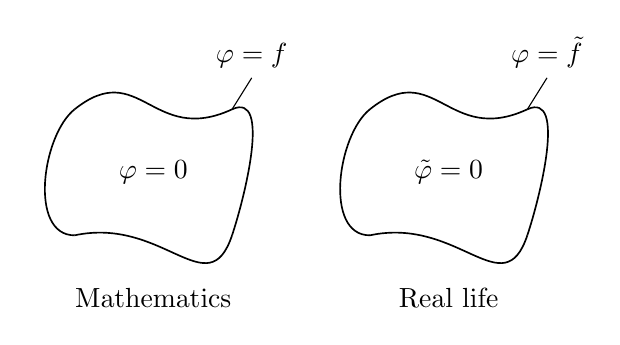
\begin{tikzpicture}[yscale=0.8]
            \node (0) at (-1, 1) {};
            \node (1) at (1, 1) {};
            \node (2) at (1, -1) {};
            \node (3) at (-1, -1) {};
            \node (4) at (0, 0) {$\laplacian \varphi=0$};
            \node (5) at (1.25, 1.5) {};
            \node [above] at (5) {$\varphi=f$};
            \node (6) at (0, -2) {Mathematics};
            \node (7) at (2.75, 1) {};
            \node (8) at (4.75, 1) {};
            \node (9) at (4.75, -1) {};
            \node (10) at (2.75, -1) {};
            \node (11) at (3.75, 0) {$\laplacian \tilde{\varphi}=0$};
            \node (12) at (5, 1.5) {};
            \node [above] at (12) {$\varphi=\tilde{f}$};
            \node (13) at (3.75, -2) {Real life};
            \draw [semithick, in=-150, out=45, looseness=1.50] (0.center) to (1.center);
            \draw [semithick, in=75, out=30, looseness=0.75] (1.center) to (2.center);
            \draw [semithick, in=15, out=-105, looseness=1.50] (2.center) to (3.center);
            \draw [semithick, in=-135, out=-180, looseness=0.75] (3.center) to (0.center);
            \draw (5.center) to (1.center);
            \draw [semithick, in=-150, out=45, looseness=1.50] (7.center) to (8.center); 
            \draw [semithick, in=75, out=30, looseness=0.75] (8.center) to (9.center);
            \draw [semithick, in=15, out=-105, looseness=1.50] (9.center) to (10.center);
            \draw [semithick, in=-135, out=-180, looseness=0.75] (10.center) to (7.center);
            \draw (12.center) to (8.center);
        \end{tikzpicture}
    \end{center}
    The error would be $ \| f-\tilde{f} \| $, which we want to be \textit{small}. i.e. we want $ \|\varphi-\tilde{\varphi}\| $ to be small. In this course we mainly care about 2.
\end{note}

We only want to solve problems that have a unique, or almost unique solution. Let us consider a generic \textit{linear} problem of the form
\[
    \begin{cases}
        L \varphi=F & \text {in } \Omega \\
        B \varphi=f & \text {on } \partial \Omega
    \end{cases} 
\]
for some \textit{linear} differential operators $L$ and $B$. If $\varphi_{1}$ and $\varphi_{2}$ are two different solutions to this problem, then their difference, $\psi=\varphi_{2}-\varphi_{1}$, must satisfy the homogeneous problem
\[
    \begin{cases}
        L \psi=0 & \text {in } \Omega \\
        B \psi=0 & \text {on } \partial \Omega
    \end{cases} 
\]
If we can show that the only solution to this problem is $\psi=0$, we will have to conclude that $\varphi_{1}=\varphi_{2},$ i.e. the solution to the original problem is unique. The moral of the story is 
\begin{quote}
    \textit{The solution to a linear problem is unique iff the only
    solution to homogeneous problem is the zero solution.}
\end{quote}

\begin{proposition}
    The solution to the Dirichlet problem is unique. The solution to the Neumann problem is unique upto addition of a constant.
\end{proposition}
\begin{proof}
    Let $ \psi=\varphi_1-\varphi_2 $ be the difference of 2 solutions to Dirichlet or Neumann problems, so 
    \[
    \begin{cases}
        \laplacian \psi=0 & \text {in } \Omega \\
        B \psi=0 & \text {on } \partial \Omega
    \end{cases} 
    \]
    where $B \psi \equiv \psi$ (Dirichlet) or $B \psi \equiv \frac{\partial \psi}{\partial \mathbf{n}}$ (Neumann). Consider the non-negative functional
    \[
        I[\psi]=\int_{\Omega}|\nabla \psi|^{2} \mathrm{~d} V \ge 0
    \]
    Clearly $I[\psi]=0$ if and only if $\nabla \psi=0$ on $\Omega$. Note that
    \[
        I[\psi]=\int_{\Omega} \nabla \psi \cdot \nabla \psi \mathrm{~d} V=\int_{\Omega}\left(\nabla \cdot(\psi \nabla \psi)-\psi \nabla^{2} \psi\right) \mathrm{d} V.
    \]
    The second term vanishes because $\nabla^{2} \psi=0$ in $\Omega$. Using the divergence theorem on the first term, we find
    \[
        I[\psi]=\int_{\partial \Omega} \psi \frac{\partial \psi}{\partial \mathbf{n}} \mathrm{~d} S=0.
    \]
    Hence $\nabla \psi=0$ throughout $\Omega,$ i.e. $\psi$ is constant. We then have two cases to consider:
    \begin{enumerate}[(a)]
        \item In the Dirichlet case, $\psi=0$ on the boundary. By continuity of $\psi$ on $\Omega \cup \partial \Omega$ we conclude $\psi=0$ throughout $\Omega$. So the solution to the Dirichlet problem is unique.
        \item In the Neumann case we only know that $\frac{\partial \psi}{\partial \mathbf{n}}=0$ on $\partial \Omega,$ so we cannot say any more than $\psi=\text{const}$ throughout $\Omega$. So the solution to the Neumann problem is unique upto the addition of a constant.\qedhere
    \end{enumerate}
\end{proof}

\begin{example}
    From electrostatics, consider charge density
    \[
        \rho(\mathbf{x}) = \begin{cases}
        0 &r<a\\
        F(r) &r\ge a\\
        \end{cases} 
    \]
    \begin{claim}
        There is no electric field in $ r<a $.
    \end{claim}
    Indeed, we know that the electric potential $ \phi $ satisfies 
    \[
        \laplacian \phi = -\frac{\rho(\mathbf{x})}{\epsilon_0}=0,\quad r<a.
    \]
    By spherical symmetry, $ \phi=\phi(r) $, so $ \phi=\phi(a)=\phi_0=\text{const} $ on $ r=a $. Note that one solution to 
    \[
        \begin{cases}
        \laplacian \phi=0 &r<a\\
        \phi=\phi_0 &r=a\\
        \end{cases} 
    \]
    is $ \phi=\phi_0 $. Since $\phi$ is constant throughout $r < a$, $\mathbf{E}(\mathbf{x}) = - \nabla \phi= \mathbf{0}$.
\end{example}

The same example holds if we replace electrostatics with gravity. We’ve essentially just proved \textbf{Newton’s shell theorem}: there is no net gravitational field anywhere inside a spherical shell. Newton’s proof was significantly more involved, but only used elementary concepts from geometry. It’s also not very rigorous.

\subsection{Gauss’ flux method}
A very clever way of getting solutions to Poisson's equation is to use the Gauss method. Suppose the source term $F$ is spherically symmetric, i.e. $F=F(r)$ where $r=|\mathbf{x}| .$ Re-write our problem as
\[
    \nabla \cdot \nabla \varphi=F(r),\quad \Omega = \mathbb{R}^{3}.
\]
Since the right hand side only depends on $r,$ the same is true of the left hand side. So we can assume $\varphi=\varphi(r)$ also, and in particular $\nabla \varphi=\varphi^{\prime}(r) \mathbf{e}_{r} .$ Integrating our equation
over a sphere of radius $R>0$ and using the divergence theorem gives
\[
    \int_{|\mathbf{x}|=R} \nabla \varphi \cdot \mathrm{d} \mathbf{S}=\int_{|\mathbf{x}|<R} F(r) \mathrm{~d} V = Q(R),
\]
where $Q(R)$ denotes the total amount of ``stuff'' with density $F(r)$ in $|\mathbf{x}|<R$.

Recall that on a sphere of radius $R$, 
\[
    \mathrm{d}\mathbf{S} = \mathbf{e}_r R^3 \sin \theta \dd \theta\dd \phi.
\]
So on $ |\mathbf{x}|=R $ we have
\begin{align*}
    \nabla \varphi \cdot \mathrm{d}\mathbf{S}&= \varphi'(r)\mathbf{e}_r \cdot (\mathbf{e}_r R^2 \sin \theta \dd \theta\dd \phi )\Big|_{|\mathbf{x}|=R}\\ 
    &= \varphi'(R)R^2 \sin \theta \dd \theta\dd \phi\\ 
    &= \varphi'(R)\dd S.
\end{align*}
Hence 
\[
    Q(R) = \int_{|\mathbf{x}|=R} \varphi'(R) \,\mathrm{d}S = \varphi'(R)\int_{|\mathbf{x}|=R}  \,\mathrm{d}S = 4\pi R^2 \varphi'(R).
\]
In summary,
\[
    \varphi'(R) = \frac{Q(R)}{4\pi R^2},\ \forall R>0 \Longrightarrow  \boxed{\nabla\varphi = \frac{Q(r)}{4\pi r^2}\mathbf{e}_r}
\]

\begin{example}
    We find the electric field produced by the spherically symmetric charge density
    \[
    \rho(r)=\begin{cases}
        \rho_{0} & 0 \le r \le a \\
        0 & r>a
    \end{cases} 
    \]
    Recall that the electric potential $\phi$ defined by $\mathbf{E}=-\nabla \phi .$ Use Maxwell's first equation
    \[
    \nabla \cdot \mathbf{E}=\frac{\rho}{\epsilon_{0}} \quad \text { i.e. } \quad \nabla^{2} \phi=-\frac{\rho}{\epsilon_{0}}.
    \]
    By the previous formula we find
    \[
    \phi^{\prime}(r)=-\frac{1}{4 \pi \epsilon_{0}} \frac{Q(r)}{r^{2}}.
    \]
    Note that if $r>a$ then $Q(r)=Q(a)=Q,$ where $Q$ denotes the total charge. We get
    \[
    \mathbf{E}(\mathbf{x})=-\phi^{\prime}(r) \mathbf{e}_{r}=\begin{cases}
        \dfrac{1}{4 \pi \epsilon_{0}} \dfrac{Q(r)}{r^{2}} \mathbf{e}_{r} & r \le a \\[10pt]
        \dfrac{1}{4 \pi \epsilon_{0}} \dfrac{Q}{r^{2}} \mathbf{e}_{r} & r>a
    \end{cases} 
    \]
    Taking $a \rightarrow 0$ we deduce that the electric field to a point charge $Q$ at the origin is
    \[
    \mathbf{E}(\mathbf{x})=\frac{Q}{4 \pi \epsilon_{0}} \frac{\mathbf{x}}{|\mathbf{x}|^{3}}.
    \]
    In this case the relevant charge density is $\rho(\mathbf{x})=Q \delta(\mathbf{x})$ and the corresponding electric
    potential is
    \[
    \phi(\mathbf{x})=\frac{Q}{4 \pi \epsilon_{0}} \frac{1}{|\mathbf{x}|}.
    \]
    Gauss' method also works if there is cylindrical symmetry. Suppose our problem takes
    the form
    \[
    \nabla^{2} \varphi=F(\rho)
    \]
    where $\rho^{2}=x^{2}+y^{2}$. We can let $ \varphi=\varphi(\rho) $, so that $ \nabla \varphi=\varphi'(\rho)\mathbf{e}_\rho $. Now 
    \[
        \int_{\partial ~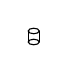
\begin{tikzpicture}[scale=0.35]
            \draw (0,0.1) ellipse (0.2 and 0.1);
            \draw (0,-0.3) ellipse (0.2 and 0.1);
            \draw (-0.2,0.1) -- (-0.2,-0.3);
            \draw (0.2,0.1) -- (0.2,-0.3); 
        \end{tikzpicture}} \nabla \varphi \cdot\mathrm{d}\mathbf{S}=\int_{~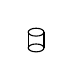
\begin{tikzpicture}[scale=0.5]
            \draw (0,0.1) ellipse (0.2 and 0.1);
            \draw (0,-0.3) ellipse (0.2 and 0.1);
            \draw (-0.2,0.1) -- (-0.2,-0.3);
            \draw (0.2,0.1) -- (0.2,-0.3); 
        \end{tikzpicture}} \div \nabla \varphi \,\mathrm{d}V = \int_{~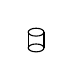
\begin{tikzpicture}[scale=0.5]
            \draw (0,0.1) ellipse (0.2 and 0.1);
            \draw (0,-0.3) ellipse (0.2 and 0.1);
            \draw (-0.2,0.1) -- (-0.2,-0.3);
            \draw (0.2,0.1) -- (0.2,-0.3); 
        \end{tikzpicture}} F(\rho) \,\mathrm{d}V.
    \]
    Note that we don't get any contribution from the ends of the cylinder because $\mathbf{n} \cdot \mathbf{e}_{\rho}=0$ on them. We have 
    \[
        \int_{\partial ~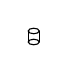
\begin{tikzpicture}[scale=0.35]
            \draw (0,0.1) ellipse (0.2 and 0.1);
            \draw (0,-0.3) ellipse (0.2 and 0.1);
            \draw (-0.2,0.1) -- (-0.2,-0.3);
            \draw (0.2,0.1) -- (0.2,-0.3); 
        \end{tikzpicture}} \nabla \varphi \cdot\mathrm{d}\mathbf{S}=\int_{\phi=0}^{2\pi} \int_{z=z_0}^{z_0+a} \varphi'(R)R \,\mathrm{d}z \,\mathrm{d}\phi = 2\pi a R \varphi'(R).
    \]
    So 
    \[
        \varphi'(R)=\frac{1}{R}\frac{1}{2\pi a}\int_{~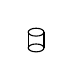
\begin{tikzpicture}[scale=0.5]
            \draw (0,0.1) ellipse (0.2 and 0.1);
            \draw (0,-0.3) ellipse (0.2 and 0.1);
            \draw (-0.2,0.1) -- (-0.2,-0.3);
            \draw (0.2,0.1) -- (0.2,-0.3); 
        \end{tikzpicture}} F(\rho) \,\mathrm{d}V=\frac{1}{R}\frac{1}{2\pi a} I,\quad \forall R>0.
    \]
    Note that 
    \[
        I = \int_{z=z_0}^{z_0+a} \int_{\phi=0}^{2\pi} \int_{\rho=0}^{R} F(\rho)\rho \,\mathrm{d}\rho \,\mathrm{d}\phi \,\mathrm{d}z = 2\pi a \int_{0}^{R} F(\rho)\rho \,\mathrm{d}\rho.
    \]
    In conclusion, 
    \[
        \boxed{\varphi'(\rho)=\frac{1}{\rho}\int_{0}^{\rho} sF(s) \,\mathrm{d}s}
    \]
\end{example}

\begin{example}
    How might we describe a \textit{line} of charge density with constant charge density $ \lambda $ per unit length?

    We could proceed as before, consider cylinder of radius $a$ with constant charge density. Take $a\to 0$ and keep charge per unit length fixed (exercise).

    Alternatively, let $ F(\rho) $ be the desired charge density. So if we integrate over \textit{any} cylinder of length 1, should have total charge contained $ \lambda $.
    \begin{align*}
        \lambda&= \int_{V} F(\rho) \,\mathrm{d}V\\ 
        &= \int_{z=z_0}^{z_0+1} \int_{\phi=0}^{2\pi} \int_{\rho=0}^{R} F(\rho)\rho \,\mathrm{d}\rho \,\mathrm{d}x \,\mathrm{d}z\\ 
        &= 2\pi \int_{0}^{R} F(\rho)\rho \,\mathrm{d}\rho .
    \end{align*}
    So we see that choosing 
    \[
        F(\rho)=\frac{\lambda \delta(\rho)}{2\pi \rho}
    \]
    the electric potential would satisfy
    \[
        \phi^{\prime}(\rho)=-\frac{1}{\epsilon_{0} \rho} \int_{0}^{\rho} \frac{\lambda}{2 \pi} \delta(s) \,\mathrm{d} s=-\frac{\lambda}{2 \pi \epsilon_{0} \rho}.
    \]
    The electric field is then
    \[
        \mathbf{E}(\mathbf{x})=\frac{\lambda}{2 \pi \epsilon_{0} \rho} \mathbf{e}_{\rho}.
    \]
\end{example}

\subsection{Superposition principle}
\textit{Linear} problems are relatively easy because of the following: 
\[
    L \psi_n = F_n,\quad n=1,2,\dots \Longrightarrow 
    L\left( \sum_{n} \psi_n \right) = \sum_{n} F_n.
\]
i.e. we can \textit{superpose} solutions. Can often break up forcing term $ F=\sum_n F_n $, solve each problem 
\[
    L \psi_n=F_n
\]
to get solution to $ L \psi=F $ with $ \psi=\sum_n \psi_n $.

\begin{example}
    Consider electric potential due to \textit{pair} of point charges $ Q_a $ at $ \mathbf{x}=\mathbf{a} $, and $ Q_b $ at $ \mathbf{x}=\mathbf{b} $. Charge densities are
    \[
        \rho(\mathbf{x})=Q_a \delta(\mathbf{x}-\mathbf{a}),\ Q_b \delta(\mathbf{x}-\mathbf{b}).
    \]
    For a point charge, the electric potential obeys 
    \[
        -\laplacian \phi = \frac{Q_a}{\epsilon_0}\delta(\mathbf{x}-\mathbf{a}).
    \]
    Solution would be 
    \[
        \phi(\mathbf{x}) = \frac{Q_a}{4\pi \epsilon_0}\frac{1}{|\mathbf{x}-\mathbf{a}|}.
    \]
    So by superposition principle, electric potential due to point charges at $ \mathbf{x}=\mathbf{a} $ and $ \mathbf{x}=\mathbf{b} $ is 
    \[
        \phi(\mathbf{x})=\frac{Q_a}{4\pi \epsilon_0}\frac{1}{|\mathbf{x}-\mathbf{a}|}+\frac{Q_b}{4\pi \epsilon_0}\frac{1}{|\mathbf{x}-\mathbf{b}|}.
    \]
\end{example}

\begin{example}
    Consider electric potential outside ball of radius $ |\mathbf{x}|<R $ of uniform charge density $ \rho_0 $. Suppose the ball has several balls removed from its interior
    \[
        |\mathbf{x}-\mathbf{a}_i|<R_i,\quad i=1,\dots,N,
    \]
    where $ |\mathbf{a}_i|+R_i<R $ and $ \forall i,j, |\mathbf{a}_i-\mathbf{a}_j|>R_i+R_j $.

    Use superposition principle: represent each hole to be a ball of uniform charge density $ -\rho_0 $. Effective potential in $ |\mathbf{x}|>R $ from each hole is 
    \[
        \phi(\mathbf{x}) = -\frac{1}{4\pi \epsilon_0}\frac{Q_i}{|\mathbf{x}-\mathbf{a}_i|},
    \]
    where $Q_{i}=\left(4 \pi R_{i}^{3} / 3\right) \rho_{0}$. Using $ Q=\left(4 \pi R^{3} / 3\right) \rho_{0} $, by superposition principle, 
    \[
        \phi(\mathbf{x})=\frac{1}{4 \pi \epsilon_{0}}\left[\frac{Q}{|\mathbf{x}|}-\sum_{i=1}^{N} \frac{Q_{i}}{\left|\mathbf{x}-\mathbf{a}_{i}\right|}\right].
    \]
\end{example}

\subsection{Integral solutions}
We know electric potential due to a point charge at $ \mathbf{x}=\mathbf{a} $ is \textit{proportional} to 
\[
    \frac{1}{|\mathbf{x}-\mathbf{a}|}
\]
We also know that a sum of point charges has, via the superposition principle, an electric potential consisting of a sum
\[
    \sum_{i=1}^{N}\frac{Q_i}{|\mathbf{x}-\mathbf{a}_i|}.
\]
This leads us to consider very general superposition of potentials of the form
\[
    \int_{\mathbb{R}^3} \frac{F(\mathbf{y})}{|\mathbf{x}-\mathbf{y}|} \,\mathrm{d}V(\mathbf{y}).
\]
\begin{proposition}
    Assume $F\to 0$ rapidly as $ |\mathbf{x}|\to \infty $. The unique solution to the Dirichlet problem
    \[
        \begin{cases}
        \laplacian\phi=F &\mathbf{x}\in\mathbb{R}^3\\
        |\phi|\to 0 &|\mathbf{x}|\to \infty\\
        \end{cases} 
    \]
    is given by 
    \[
        \phi(\mathbf{x}) = -\frac{1}{4\pi}\int_{\mathbb{R}^3} \frac{F(\mathbf{y})}{|\mathbf{x}-\mathbf{y}|} \,\mathrm{d}V(\mathbf{y}).
    \]
\end{proposition}

This result is equivalent to saying
\[
    \nabla^{2}\left(-\frac{1}{4 \pi} \frac{1}{|\mathbf{x}|}\right)=\delta(\mathbf{x})
\]
since by differentiating (with respect to the $\mathbf{x}$-variables) under the integral sign
\[
    \int_{\mathbb{R}^{3}} \nabla^{2}\left(-\frac{1}{4 \pi} \frac{1}{|\mathbf{x}-\mathbf{y}|}\right) F(\mathbf{y}) \,\mathrm{d} V=\int_{\mathbb{R}^{3}} \delta(\mathbf{x}-\mathbf{y}) F(\mathbf{y}) \,\mathrm{d} V=F(\mathbf{x})
\]

You can prove this rigorously on Example Sheet 3, on one of the additional problems. Using suffix notation and Cartesian coordinates we have for $r \neq 0$
\[
\frac{\partial^{2}}{\partial x_{i} \partial x_{i}}\left(\frac{1}{r}\right)=\frac{\partial}{\partial x_{i}}\left(-\frac{x_{i}}{r^{3}}\right)=-\frac{\delta_{i i}}{r^{3}}+\frac{3 x_{i} x_{i}}{r^{5}}=0.
\]
So certainly
\[
\nabla^{2}\left(-\frac{1}{4 \pi} \frac{1}{|\mathbf{x}|}\right)=\delta(\mathbf{x}) \quad \text { for } \mathbf{x} \neq \mathbf{0}.
\]
If we assume the divergence theorem works with $ \delta $ functions, then for any ball $|\mathbf{x}|<R$
\[
\begin{aligned}
\int_{|\mathbf{x}|<R} \nabla^{2}\left(\frac{1}{|\mathbf{x}|}\right) \mathrm{d} V &=\int_{|\mathbf{x}|=R} \nabla\left(\frac{1}{r}\right) \cdot \mathrm{d} \mathbf{S} \\
&=\int_{\theta=0}^{\pi} \int_{\phi=0}^{2 \pi}\left(-\frac{\mathbf{e}_{r}}{R^{2}}\right) \cdot \mathbf{e}_{r} R^{2} \sin \theta \,\mathrm{d} \phi \,\mathrm{d} \theta \\
&=-4 \pi.
\end{aligned}
\]
So for any $R>0$ we have
\[
\int_{|\mathbf{x}|<R} \nabla^{2}\left(-\frac{1}{4 \pi} \frac{1}{|\mathbf{x}|}\right) \mathrm{d} V=1=\int_{|\mathbf{x}|<R} \delta(\mathbf{x}) \,\mathrm{d} V.
\]
This is exactly the same behaviour as the delta function $\delta(\mathbf{x}) .$ So we conclude
\[
\nabla^{2}\left(-\frac{1}{4 \pi} \frac{1}{|\mathbf{x}|}\right)=\delta(\mathbf{x})
\]
and the result in the proposition follows. This is an example of a Green's function. You will see a lot more of these in the IB Methods.

\subsection{Harmonic functions}
\begin{definition}[harmonic functions]
    Recall that when the forcing term in Poisson's equation $ F=0 $, we call it Laplace's equation $ \laplacian \varphi=0 $. Solutions to Laplace's equation are called \textbf{harmonic functions}.
\end{definition}
\begin{proposition}[Mean Value Theorem/Property]
    If $ \varphi $ is harmonic on $ \Omega \subseteq \mathbb{R}^3 $, then 
    \[
        \varphi(\mathbf{a}) = \frac{1}{4\pi r^2} \int_{|\mathbf{x}-\mathbf{a}|=r} \varphi(\mathbf{x}) \,\mathrm{d}S
    \]
    for $ \mathbf{a}\in \Omega $ and $r$ sufficiently small so that the ball $ |\mathbf{x}-\mathbf{a}| $ is in $ \Omega $.
\end{proposition}
\begin{note}
    This says that $ \varphi(\mathbf{a}) $ can be evaluated as a mean of the values on the ball $ |\mathbf{x}-\mathbf{a}|=r $.
\end{note}
\begin{proof}
    Let $ F(r)=\text{RHS} $. Then 
    \begin{align}
        F(r) &= \frac{1}{4\pi r^2} \int_{|\mathbf{x}|=r} \varphi(\mathbf{a}+\mathbf{x}) \,\mathrm{d}S\nonumber\\ \nonumber
        &= \frac{1}{4\pi r^2} \int_{\phi=0}^{2\pi} \int_{\theta=0}^{\pi} \varphi(\mathbf{a}+r\mathbf{e}_r) r^2 \sin \theta \,\mathrm{d}\theta \,\mathrm{d}\phi\\ 
        &= \frac{1}{4\pi} \int_{\phi=0}^{2\pi} \int_{\theta=0}^{\pi} \varphi(\mathbf{a}+r\mathbf{e}_r) \sin \theta \,\mathrm{d}\theta \,\mathrm{d}\phi.\tag{$*$}
    \end{align}
    Compute $ F'(r) $: 
    \begin{align*}
        F'(r)&= \frac{1}{4\pi r^2}\int_{\phi=0}^{2\pi} \int_{\theta=0}^{\pi} \mathbf{e}_r \cdot \nabla \varphi(\mathbf{a}+r\mathbf{e}_r) r^2 \sin \theta \,\mathrm{d}\theta \,\mathrm{d}\phi\\ 
        &= \frac{1}{4\pi r^2} \int_{|\mathbf{x}|=r} \nabla \varphi(\mathbf{a}+r\mathbf{e}_r) \cdot \mathbf{e}_r \,\mathrm{d}S\\ 
        &= \frac{1}{4\pi r^2} \int_{|\mathbf{x}-\mathbf{a}|=r} \nabla \varphi(\mathbf{x})  \cdot \mathrm{d}\mathbf{S} = \frac{1}{4\pi r^2} \int_{|\mathbf{x}-\mathbf{a}|<r} \laplacian \varphi(\mathbf{x}) \,\mathrm{d}V\\ 
        & =0.
    \end{align*}
    So $F(r)$ is constant. Take $ r\to 0 $ in ($ * $) we have $ F(r)=\varphi(\mathbf{a}) $, as claimed.
\end{proof}

Using idea in the proof, we can deduce what Laplacian is \textit{actually} meaning:
\begin{proposition}
    For any smooth $ \varphi: \mathbb{R}^{3}\to \mathbb{R} $, we have 
    \[
        \nabla^{2} \varphi(\mathbf{a})=\lim _{r \rightarrow 0} \frac{6}{r^{2}}\left[\frac{1}{4 \pi r^{2}} \int_{|\mathbf{x}-\mathbf{a}|=r} \varphi(\mathbf{x})\, \mathrm{d} S-\varphi(\mathbf{a})\right].
    \]
    In particular, \textit{$ \varphi $ is harmonic if and only if $ \varphi $ has the mean value property.}
\end{proposition}
\begin{proof}
    Define 
    \[
        G(r) = \frac{1}{4 \pi r^{2}} \int_{|\mathbf{x}-\mathbf{a}|=r} \varphi(\mathbf{x})\, \mathrm{d} S-\varphi(\mathbf{a}).
    \]
    i.e. $G$ measures the error of $ \varphi(\mathbf{a}) $ to its average. From the previous proof,
    \[
        G'(r) = F'(r) = \frac{1}{4\pi r^2} \int_{|\mathbf{x}-\mathbf{a}|<r} \laplacian \varphi(\mathbf{x}) \,\mathrm{d}V,
    \]
    which will vanish if $ \varphi $ is harmonic. Note that we can approximate the integral as
    \begin{align*}
        \int_{|\mathbf{x}-\mathbf{a}|<r} &\laplacian \varphi(\mathbf{x}) \,\mathrm{d}V \\
        &= \laplacian \varphi(\mathbf{a})\int_{|\mathbf{x}-\mathbf{a}|<r} \,\mathrm{d}V + \int_{|\mathbf{x}-\mathbf{a}|<r} \left( \laplacian \varphi(\mathbf{x})-\laplacian \varphi(\mathbf{a}) \right) \,\mathrm{d}V\\ 
        &= \frac{4\pi}{3}r^3\laplacian \varphi(\mathbf{a})+ o(r^3) \quad\left(r \to 0\right)
    \end{align*} 
    where the $o$ term comes from the fact that
    \[
        \begin{aligned}
            &\left|\int_{|\mathbf{x}-\mathbf{a}|<r}\left(\nabla^{2} \varphi(\mathbf{x})-\nabla^{2} \varphi(\mathbf{a})\right) \,\mathrm{d} V\right|\\ 
             \le& \sup _{|\mathbf{x}-\mathbf{a}|<r}\left|\nabla^{2} \varphi(\mathbf{x})-\nabla^{2} \varphi(\mathbf{a})\right| \int_{|\mathbf{x}-\mathbf{a}|<r} \mathrm{~d} V \\
            =&\sup _{|\mathbf{x}-\mathbf{a}|<r}\left|\nabla^{2} \varphi(\mathbf{x})-\nabla^{2} \varphi(\mathbf{a})\right|\left(\frac{4 \pi r^{3}}{3}\right).
        \end{aligned}
    \]
    So 
    \begin{align*}
        G'(r) &= \frac{1}{4\pi r^2}\int_{|\mathbf{x}-\mathbf{a}|<r} \laplacian \varphi(\mathbf{x}) \,\mathrm{d}V\\ 
        &= \frac{1}{4\pi r^2}\left( \frac{4\pi}{3}r^3\laplacian \varphi(\mathbf{a})+ o(r^3) \right)\\ 
        &= \frac{r}{3}\laplacian \varphi(\mathbf{a})+o(r) \quad\left(r \to 0\right).
    \end{align*}
    Consider the Taylor expansion of $ G'(r) $ near 0:
    \[
        G'(r) = G'(0)+rG''(r)+o(r) \quad\left(r \to 0\right),
    \]
    we deduce that 
    \[
        G'(0)=0,\quad G''(z) = \frac{1}{3}\laplacian \varphi(\mathbf{a}).
    \]
    Hence 
    \begin{align*}
        G(r) &= G(0) + r G'(0) + \frac{r^2}{2}G''(0)+ o(r^2)\\ 
        &= \frac{r^2}{6}\laplacian \varphi(\mathbf{a}) + o(r^2) \quad\left(r \to 0\right).
    \end{align*}
    Hence 
    \[
        \laplacian\varphi(\mathbf{a}) = \lim_{r \to 0} \frac{6}{r^2}G(r)=\lim _{r \rightarrow 0} \frac{6}{r^{2}}\left[\frac{1}{4 \pi r^{2}} \int_{|\mathbf{x}-\mathbf{a}|=r} \varphi(\mathbf{x})\, \mathrm{d} S-\varphi(\mathbf{a})\right].\qedhere
    \]
\end{proof}

\begin{proposition}[Maximum Principle]
    If $ \varphi $ is harmonic on $ \Omega \subseteq \mathbb{R}^{3} $, then $ \varphi $ cannot have a maximum at any interior point of $ \Omega $ unless $ \varphi $ is constant.
\end{proposition}
\begin{proof}
    Suppose $ \mathbf{a} $ is an interior point of $ \Omega $ such that $ \forall \mathbf{x}\in \Omega,\ \varphi(\mathbf{a})\ge \varphi(\mathbf{x}) $. In particular, $ \exists \epsilon>0 $ such that $ \varphi(\mathbf{a})\ge \varphi(\mathbf{x}),\ 0<|\mathbf{x}-\mathbf{a}|\le\epsilon $. By MVT, 
    \[
        \varphi(\mathbf{a}) = \frac{1}{4\pi \epsilon^2}\int_{|\mathbf{x}-\mathbf{a}|=\epsilon} \varphi(\mathbf{x}) \,\mathrm{d}S \Longrightarrow \frac{1}{4\pi \epsilon^2}\int_{|\mathbf{x}-\mathbf{a}|=\epsilon} \varphi(\mathbf{a})-\varphi(\mathbf{x}) \,\mathrm{d}S=0.
    \]
    Since $ \varphi(\mathbf{a})-\varphi(\mathbf{x})\ge 0 $, we have $ \varphi(\mathbf{a})=\varphi(\mathbf{x}) $ on $ |\mathbf{x}-\mathbf{a}|=\epsilon $. Since this also works for all $ \epsilon'<\epsilon $, we conclude that $ \varphi(\mathbf{x})=\varphi(\mathbf{a}) $ on $ |\mathbf{x}-\mathbf{a}|\le \epsilon $.

    Now pick any other point $\mathbf{y} \in \Omega$. Connect $\mathbf{a}$ to $\mathbf{y}$ with a bunch of overlapping balls such that the center of the $(n+1)$ th ball is contained in the $n$ th. On the first ball we know $\varphi(\mathbf{x})=\varphi(\mathbf{a})$. On the center of the second ball we must also have $\varphi(\mathbf{x})=\varphi(\mathbf{a})$, and so this holds all throughout the second ball by our previous argument. Continuing inductively we get that $\varphi(\mathbf{x})=\varphi(\mathbf{a})$ on a ball containing $\mathbf{y}$. So $\varphi(\mathbf{a})=\varphi(\mathbf{y}),$ and since $\mathbf{y} \in \Omega$ is arbitrary we conclude that $\varphi$ is constant throughout $\Omega$\footnote{There is a little concersquen about whether or not we’d have to keep making the balls smaller and smaller, so much so that we could never get to $\mathbf{y}$. This issue can be dealt with once you have learnt about \textit{compactness} in Metric \& Topological spaces. Our proof can be made rigorous with a couple of easy tweaks.}.
\end{proof}
\begin{proof}[Alternatively,]
    Consider $ U \subseteq \Omega $ such that $ U=\{\mathbf{x}\in \Omega: \varphi(\mathbf{x})=\varphi(\mathbf{a})\} $. It is non-empty, open by MVT, and closed by continuity of $ \varphi $. So $ U=\Omega $. See Analysis and Topology.
\end{proof}
Immediately,
\begin{corollary}
    If $ \varphi $ is harmonic on $ \Omega $, then 
    \[
        \varphi(\mathbf{x}) \le \max _{\mathbf{x} \in \partial \Omega} \varphi(\mathbf{x}).
    \]
\end{corollary}

\subsection{Discrete Laplacian and Liouville’s theorem}
We've seen that the Laplacian of a function at $\mathbf{x}=\mathbf{a}$ can be thought of as measure of how much a function differs from its average on points around a. A natural definition of the Laplacian of a function on $\mathbb{Z}^{n}$ would be
\[
\nabla^{2} \varphi(\mathbf{d}):=\frac{\sum_{i=1}^{n} \varphi\left(\mathbf{d}+\mathbf{e}_{i}\right)+\sum_{i=1}^{n} \varphi\left(\mathbf{d}-\mathbf{e}_{i}\right)}{2 n}-\varphi(\mathbf{d}).
\]
where $\mathbf{e}_{i}$ are the standard Cartesian basis vectors. For example on $\mathbb{Z}^{2}$, $ \forall (i, j) \in \mathbb{Z}^{2} $ we have
\[
    \nabla^{2} \varphi(i, j)=\frac{\varphi(i+1, j)+\varphi(i, j+1)+\varphi(i-1, j)+\varphi(i, j-1)}{4}-\varphi(i, j).
\]
Liouville's theorem for the discrete Laplcian is as follows.

\begin{theorem}[Liouville]
    If $\varphi: \mathbb{Z}^{n} \rightarrow \mathbb{Z}$ is bounded and $\nabla^{2} \varphi=0$ then $\varphi=$ const.
\end{theorem}

\begin{proof}
    If $\varphi$ is bounded, then the set $\left\{\varphi(\mathbf{d}), \mathbf{d} \in \mathbb{Z}^{n}\right\}$ is finite and has a least element, $\alpha$ say. Suppose $\varphi(\mathbf{d})=\alpha$. Then either all the $\varphi\left(\mathbf{d} \pm \mathbf{e}_{i}\right)$ are the same, or at least one is less than $\alpha$ since $\nabla^{2} \varphi=0 .$ The latter can't happen, so we must have $\varphi\left(\mathbf{d} \pm \mathbf{e}_{i}\right)=\alpha$. Carrying on in this fashion we see that $\varphi(\mathbf{d})=\alpha$ for each $\mathbf{d} \in \mathbb{Z}^{n}$.
\end{proof}

\begin{sque}
    Does the statement of the theorem remain true if $\varphi: \mathbb{Z}^{n} \rightarrow \mathbb{Z}$ is replaced with $\varphi: \mathbb{Z}^{n} \rightarrow \mathbb{R} ?$
\end{sque}